\documentclass[tikz,border=10pt]{standalone}
\usepackage{tikz}
\usetikzlibrary{arrows.meta,positioning}

\tikzset{
  block/.style={draw=blue!70!black, line width=1.2pt, minimum width=2.2cm, minimum height=1.0cm, align=center, fill=none},
  sum/.style={circle, draw=green!50!black, line width=1.2pt, minimum size=7mm, inner sep=0pt},
  card/.style={draw=orange!80!black, line width=1.2pt, rounded corners=3pt, minimum width=3.0cm, minimum height=0.95cm, align=center, fill=none},
  signal/.style={-{Stealth[length=3mm]}, line width=1.2pt, draw=black!70}
}

\begin{document}
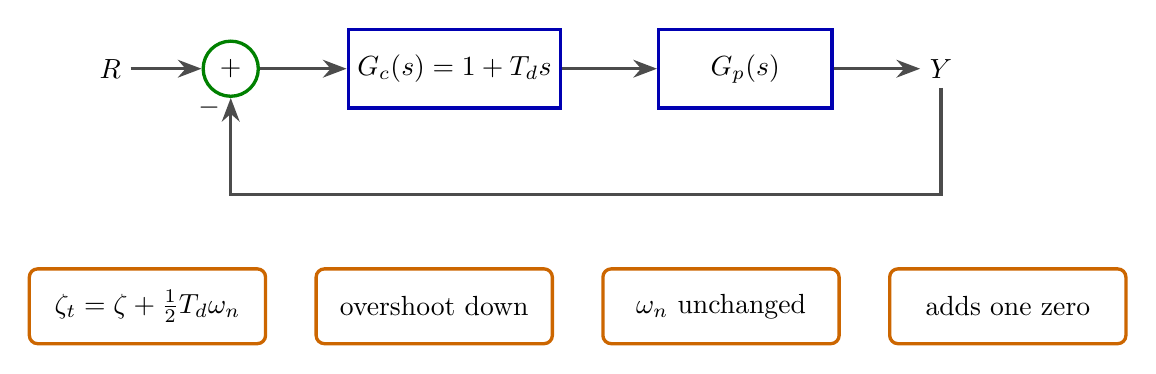
\begin{tikzpicture}[node distance=1.0cm and 1.0cm]
  \node (r) {$R$};
  \node[sum, right=0.9cm of r] (sum1) {$+$};
  \node[block, right=1.1cm of sum1] (gc) {$G_c(s)=1+T_d s$};
  \node[block, right=1.2cm of gc] (gp) {$G_p(s)$};
  \node[right=1.1cm of gp] (y) {$Y$};

  \draw[signal] (r) -- (sum1);
  \draw[signal] (sum1) -- (gc);
  \draw[signal] (gc) -- (gp);
  \draw[signal] (gp) -- (y);
  \draw[signal] (y) |- ++(0,-1.6) -| node[pos=0.95,left] {$-$} (sum1.south);

  \node[card, below=2.0cm of gc, xshift=-3.9cm] (c1) {$\zeta_t = \zeta + \frac{1}{2} T_d \omega_n$};
  \node[card, right=0.6cm of c1] (c2) {overshoot down};
  \node[card, right=0.6cm of c2] (c3) {$\omega_n$ unchanged};
  \node[card, right=0.6cm of c3] (c4) {adds one zero};
\end{tikzpicture}
\end{document}
